%\documentclass[preprint,3p,times,twocolumn]{elsarticle}
\documentclass[review,3p,times]{elsarticle}
\usepackage{amssymb}
\usepackage{amsmath}
\usepackage{graphicx}
\usepackage{bm}
\usepackage{yhmath}
\usepackage{subfigure}
\usepackage{multirow}
\usepackage{cleveref}
\usepackage{xcolor}
%\definecolor{}{rgb}{0,0,255}
\usepackage{subdepth}
%\usepackage[nomarkers,lists]{endfloat}

\def\pp#1#2{\frac{\partial #1}{\partial #2}}

\biboptions{comma,sort&compress}

\journal{Proceedings of Combustion Institute}

\makeatletter
\def\@author#1{\g@addto@macro\elsauthors{\normalsize%
    \def\baselinestretch{1}%
    \upshape\authorsep#1\unskip\textsuperscript{%
      \ifx\@fnmark\@empty\else\unskip\sep\@fnmark\let\sep=,\fi
      \ifx\@corref\@empty\else\unskip\sep\@corref\let\sep=,\fi
      }%
    \def\authorsep{\unskip,\space}%
    \global\let\@fnmark\@empty
    \global\let\@corref\@empty  %% Added
    \global\let\sep\@empty}%
    \@eadauthor={#1}
}
\makeatother

\begin{document}

\begin{frontmatter}

\title{Flame dynamics in oscillating flows under autoignitive conditions}

\author[Princeton]{Sili~Deng\corref{cor}}
\author[Princeton,Oakland]{Peng~Zhao}
\author[Princeton]{Michael E.~Mueller}
\author[Princeton]{Chung K.~Law}
\cortext[cor]{Corresponding Author: silideng@princeton.edu}

\address[Princeton]{Department of Mechanical and Aerospace Engineering, Princeton University, Princeton, NJ 08544, USA}
\address[Oakland]{Department of Mechanical Engineering, Oakland University, Rochester, MI 48309, USA}

\begin{abstract}

The structure and dynamics of laminar nonpremixed dimethyl ether (DME)/air coflow flames were investigated at elevated temperatures and pressures.  Computations with detailed chemistry were performed for DME and heated coflow air at $30$ atm with uniform but sinusoidally oscillating inlet velocities.  These unsteady cases were compared with the steady results from Deng~\emph{et al.} (\emph{Combust. Flame}, in press) to elucidate the effect of oscillation frequency on the flame dynamics.  To benchmark the unsteady cases, a normalized displacement velocity was defined to differentiate flame propagation from autoignition, and this definition was validated against the steady cases.  In the oscillating reacting flow, transition between a multibrachial autoignition front and a tribrachial flame occurs periodically.  However, unlike the harmonic velocity oscillation, the combustion mode transition is hysteretic.  The oscillation cycle starts with the largest inlet velocity, with the multibrachial thermal structure, located downstream, being governed by autoignition chemistry.  As flow velocity decreases, the autoignition front moves upstream and transitions to a tribrachial flame near the lower velocity limit, similar to the steady flow, as autoignition chemistry becomes weaker with decreasing upstream residence time.  As the flow velocity increases again, the tribrachial flame is convected downstream, and, ultimately, due to the radical and heat accumulation in time, autoignition eventually occurs and becomes the dominant pathway.  The finite induction time for autoignition results in the hysteretic behavior during the decreasing and increasing-velocity cycles, which diminishes at lower oscillation frequency as there is more time for chemistry to respond to the hydrodynamic changes and consequently approach steady state.  

\end{abstract}

\begin{keyword} 
Flame dynamics \sep Nonpremixed coflow flame \sep Autoignition \sep Negative temperature coefficient (NTC) \sep Dimethyl ether (DME) 
\end{keyword}

\end{frontmatter}


%\clearpage % For word count
%==============================================================

\section{Introduction}

Fuel injection and its subsequent mixing and reaction with either a coflowing air stream or a highly turbulent oxidizing environment is an integral process in the operation of many combustors.  Due to experimental and computational limitations, simplifications are usually made to obtain fundamental understanding of these reacting flows that are then extrapolated to more complex conditions.  For example, laminar nonpremixed coflow flames at normal ambient temperatures have been studied to elucidate the coupling between fluid dynamics and chemistry, leading to the observation that, in the fuel and oxidizer mixing layer, a two-dimensional tribrachial structure (also known as triple flame)~\cite{buckmaster02} is obtained.  Specifically, both lean and rich premixed flame branches and a trailing diffusion flame tail intersect at a triple point.  Based on the observation of such tribrachial laminar flames, the partially premixed flamelet model~\cite{muller94} was proposed to explain lifted flames in nonpremixed turbulent jets~\cite{chung07}.

Previous studies have indicated that this classical tribrachial flame structure can be modified in unsteady flows.  For example, in the experimental investigation of Strawa and Cantwell~\cite{strawa89}, flow instability and flame breakup was achieved by imposing a small-amplitude, periodic velocity fluctuation to nonpremixed jet flames at elevated pressures and low Reynolds numbers.  Later, in the computational study of S\'{a}nchez-Sanz~\emph{et al.}~\cite{sanchezsanz10}, perturbation frequency effects on the thermal and chemical properties of the flame in such periodically time-varying flows were evaluated.  Three regimes were found depending on the flame's Strouhal number, $S = af/U$, with $a$ and $f$ denoting the fuel jet radius and perturbation frequency, respectively.  For small Strouhal numbers ($S = 0.1$), perturbations can travel far downstream, resulting in an oscillating flame.  Flame surface flickering was observed when $S\simeq 0.2$, and vigorous flame pinch-off was observed at $S = 0.5$.  Larger values of $S$ confine the oscillation to the jet's near-exit region, and the pulsation has minimal effects on temperature and concentration values.

The unsteadiness in flickering flames also increases pollutant formation, such as soot~\cite{shaddix94} and carbon monoxide~\cite{skaggs96}.  Mohammed~\emph{et al.}~\cite{mohammed98} followed by Dworkin~\emph{et al.}~\cite{dworkin07} conducted computational and experimental studies of $20$ Hz periodically-forced methane/air coflow diffusion flames.  Acetylene production increased~\cite{mohammed98} and the oxidation of CO to CO$_2$ was inhibited~\cite{dworkin07} in the downstream region of the flame at certain times during the flame's cyclic history.       

Although demonstrating unsteady effects on flow-chemistry coupling, these experimental and computational investigations mainly focused on simple fuels, such as methane, and were limited to nonautoignitive conditions.  Under more realistic engine conditions of elevated temperature and pressure with practical fuels that have more complex chemical kinetics, more complicated transport-chemistry coupling has been observed.  For example, Krisman~\emph{et al.}~\cite{krisman14} first computationally demonstrated that, besides the traditional tribrachial flame, autoignition is also a relevant combustion process or even the dominant one under certain conditions.  Their findings were confirmed and further discussed by Deng~\emph{et al.}~\cite{deng15,deng15b} through a series of computational studies of nonpremixed dimethyl ether (DME)/air coflow flames at $30$ atm with varying inlet velocities and coflow temperatures, recognizing that DME possesses the low-temperature chemistry (LTC), negative temperature coefficient (NTC) behavior.  A regime diagram was proposed demonstrating that the tribrachial flame is favored at lower inlet velocity and higher coflow temperature, while autoignition is dominant at higher inlet velocity and relatively lower coflow temperature.

In the present study, unsteady nonpremixed DME/air coflow flames under autoignitive conditions are computationally studied to elucidate the coupling between unsteady fluid dynamics and chemical kinetics.  Various oscillation frequencies were imposed on the inlet velocity, with the maximum and minimum velocities maintained the same as those in the previous steady study~\cite{deng15b}, which correspond to an autoignition front and a tribrachial flame, respectively.  The objective of the current study is threefold.  The first objective is to capture the transition in combustion mode.  As the steady cases correspond to different combustion modes, it is expected that, at certain frequencies of velocity oscillation, the dominant combustion process will shift between the nonpremixed tribrachial flame mode and the autoignition mode.  The second objective is to assess the thermal and chemical differences during such transition and to elucidate the transition mechanism.  The third objective is to demonstrate the effects of oscillation frequency on the coupling of fluid dynamics and chemical kinetics.               

 
%===============================================================

\section{Computational details} \label{sec:computation}

The geometry in this work is the same as that in Deng~\emph{et al.}~\cite{deng15b}.  Briefly, axisymmetric coflow flames at $30$ atmospheres were computed, in which a $300$ K DME stream is surrounded by a $900$ K air stream.  The diameter ($D$) of the fuel nozzle is $0.8$ mm, which is $20$ times the thickness of the adiabatic, no-slip wall, separating fuel and coflow.  The outer diameter of the coflow is $3.9$ mm.  Adiabatic, slip wall conditions were specified at the outer radial boundary.  The same inlet velocities were imposed for both streams and are uniform in space and sinusoidally oscillating in time.  The maximum ($8.0$ m/s) and minimum ($2.4$ m/s) velocities were set to match the fastest and slowest steady cases as in Deng~\emph{et al.}~\cite{deng15b}.  Three oscillation frequencies ($25$, $50$, and $100$ Hz) were investigated, with the maximum Strouhal number, based on the velocity and jet radius, estimated to be less than $0.02$ to avoid flame pinch-off.  The domain length is $15$ mm, with a convective outflow boundary condition.  The computational results were not affected by further widening or lengthening of the domain.  Discretization of the domain was guided by previous convergence studies~\cite{deng15}, with a $3072$ ($x$) by $176$ ($r$) grid.  Uniform spacing in the axial direction was set to $\Delta x = 4.8$ ${\rm \mu}$m, and nonuniform spacing in the radial direction was set to minimum $\Delta r = 2.5$ ${\rm \mu}$m to resolve the mixing layer near the thin wall.  The grid stretch rate is less than $3$\%.

The Navier-Stokes equations with buoyancy effects in the streamwise direction and the conservation equations of mass, species, and temperature were solved.  The species diffusivities were determined assuming constant, nonunity Lewis numbers and kept the same as in Deng~\emph{et al.}~\cite{deng15}.  The conserved scalar mixture fraction ($Z$) was specified as unity and zero for the fuel stream and coflow, respectively, and was computed by solving a conserved scalar transport equation with unity Lewis number~\cite{pitsch98b}.  DME was chosen as the fuel, for it is one of the simplest fuels that has NTC chemistry~\cite{deng14}, as noted earlier.  A skeletal mechanism of $39$ species~\cite{bhagatwala15}, which was reduced from the well-validated detailed mechanism of Zhao \emph{et al.}~\cite{zhao08}, was adopted as the chemical model.    

A low-Mach number code NGA~\cite{desjardins08} was adopted to solve the discretized governing equations on a staggered mesh.  A second-order centered scheme was used for the momentum equations, while a third-order WENO scheme~\cite{liu94} was used for the scalar equations.  An iterative second-order semi-implicit midpoint scheme was adopted for temporal integration~\cite{pierce01} utilizing Strang splitting between transport and chemistry in the scalar equations.  The chemical source terms for the species and temperature equations were integrated using the CVODE package~\cite{cohen96}.

%===============================================================

\section{Results and discussion}

In this section, the thermal structure of the unsteady nonpremixed DME/air coflow flame is first described and compared qualitatively with the previous steady study by Deng~\emph{et al.}~\cite{deng15b}.  The definition of normalized displacement velocity is then introduced and validated against the steady cases to differentiate the combustion modes.  Finally, oscillation frequency effects on the evolution of the combustion modes are analyzed.   

\subsection{Thermal structure}

As the largest and smallest inlet velocity cases were designed to match the two extreme cases in Deng~\emph{et al.}~\cite{deng15b}, which are of different thermal structures, it is expected that similar thermal structures will be obtained.  Furthermore, these thermal structures might transition back and forth in response to the oscillating flow field.  Indeed, such transitions were observed for all three frequencies.  For example, the evolution of the thermal structure of the $100$ Hz case, in terms of the heat release rate profile, is demonstrated in Fig.~\ref{fig:HRR_100Hz}.  The oscillation cycle starts with the largest inlet velocity of $8.0$ m/s, and the minimum inlet velocity ($2.4$ m/s) is achieved at half cycle.  

\begin{figure*}[t]
  \centering
  \scriptsize
  \vspace{-0.10in}
  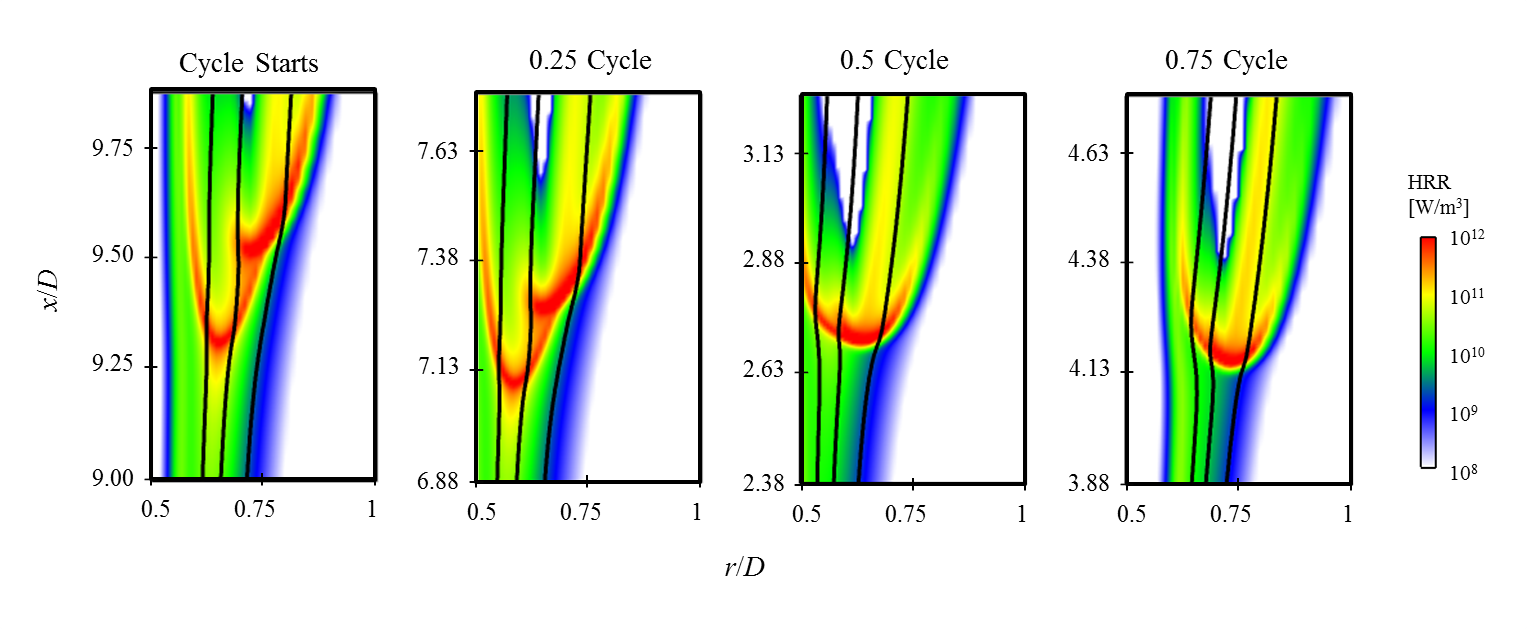
\includegraphics[trim=6.5mm 7.5mm 7mm 8mm, clip=true, width=1.0\textwidth]{HRR_100Hz.png}
  \normalsize
  \vspace{-0.2in}
  \caption{Heat release rate [W/m$^3$] profile evolution during one oscillation cycle at $100$ Hz.  The iso-contours of $Z_{\rm st} = 0.1$, $Z = 0.2$, and $Z = 0.3$ are outlined from right to left in solid lines, respectively.}
  \label{fig:HRR_100Hz}
\end{figure*}


At $8.0$ m/s, the multibrachial thermal structure is located furthest downstream.  The leading point, which is defined as the most upstream point that has the heat release rate value of $10^{12}$ W/m$^3$, is located at mixture fraction $Z = 0.24$.  As the inlet velocity decreases, the multibrachial structure moves upstream, without obvious change of the leading point location, in terms of mixture fraction.  When the inlet velocity reaches its minimum, the multibrachial structure transitions to a tribrachial structure, and the leading point switches to $Z = 0.14$.  As the flow velocity increases, the tribrachial structure is pushed downstream, and both its tribrachial shape and its leading point mixture fraction remain unchanged.  The thermal structure returns to that of multibrachial when the flow velocity further increases.  Such transitions in structure repeat once a new oscillation cycle starts.

\subsection{Differentiation of combustion mode}

As mentioned in the Introduction, Deng~\emph {et al.}~\cite{deng15b} were able to relate the morphology of the thermal structures to two different combustion modes: tribrachial flame and autoignition.  Specifically, at steady state, the multibrachial structure in the $8.0$ m/s case is an autoignition front, while the $2.4$ m/s case is a tribrachial flame.  In this previous study, species mass fraction profiles at the inlet of the two-dimensional computation were treated as the initial conditions for one-dimensional Lagrangian Flamelet Analysis~\cite{pitsch98a}, which only considers diffusion processes parallel to the mixture fraction gradient and neglects those in the normal direction.  When the LFA prediction agreed with the CFD result, transport in the normal direction of the mixture fraction gradient was negligible, and autoignition was the dominant combustion process.  However, due to the unsteadiness in the current study, such comparison between LFA and CFD is no longer applicable, and a new criterion to differentiate the modes of tribrachial flame and autoignition needs to be identified and validated against the steady cases.

A density-weighted displacement speed, $S_d$, is often used to distinguish between deflagrations and spontaneous ignition fronts in HCCI combustion~\cite{yoo13}, which is defined from an iso-line of species $k$ as~\cite{ruetsch95,im99}:

\begin{equation} \label{eq:sd}
S_d = \frac{1}{\rho{_u} |\nabla Y_k|} \left(\dot{\omega}{_k} - \pp{\rho Y_k V_{j,k}}{x_j} \right),
\end{equation}
where $Y_k$, $V_{j,k}$, and $\dot{\omega}{_k}$ denote species mass fraction, diffusion velocity in the $j$-direction, and net production rate, respectively, and $\rho {_u}$ is the density of the unburnt mixture.  The choice of species $k$ and its iso-line value can be ambiguous.  Therefore, major products, such as CO$_2$, H$_2$O, H$_2$, CO, and combinations of these products have been tested, and the sampling location is chosen as the leading point, as defined above, to enable further comparison with the steady cases.  $S_d$ at the leading point is insensitive to the choice of species in the current study, for less than $5$\% difference was observed across all the combinations.  Consequently, H$_2$O was chosen for simplicity.  Both the laminar flame speed $S_L$ and the unburnt mixture density $\rho {_u}$ were obtained from laminar flame speed calculations using the FlameMaster code~\cite{flamemaster}.  The composition and temperature boundary conditions for the laminar flame speed calculations were based on the sampled mixture fraction at the leading point and linearly interpolated, in the mixture fraction space, between the corresponding inlet values of the fuel and coflow streams.  

Following the above procedure, displacement velocities were calculated for all three oscillation frequency cases, with $20$ points per cycle, to demonstrate their evolution.  Furthermore, as shown in Fig.~\ref{fig:sd_evo}, $S_d/S_L$ for the two steady cases ($2.4$ and $8.0$ m/s) were similarly calculated to validate this definition of normalized displacement velocity and differentiate between tribrachial flame and autoignition.

\begin{figure}[t]
  \centering
  \scriptsize
  \resizebox{0.5\textwidth}{!}{% GNUPLOT: LaTeX picture with Postscript
\begingroup
  \makeatletter
  \providecommand\color[2][]{%
    \GenericError{(gnuplot) \space\space\space\@spaces}{%
      Package color not loaded in conjunction with
      terminal option `colourtext'%
    }{See the gnuplot documentation for explanation.%
    }{Either use 'blacktext' in gnuplot or load the package
      color.sty in LaTeX.}%
    \renewcommand\color[2][]{}%
  }%
  \providecommand\includegraphics[2][]{%
    \GenericError{(gnuplot) \space\space\space\@spaces}{%
      Package graphicx or graphics not loaded%
    }{See the gnuplot documentation for explanation.%
    }{The gnuplot epslatex terminal needs graphicx.sty or graphics.sty.}%
    \renewcommand\includegraphics[2][]{}%
  }%
  \providecommand\rotatebox[2]{#2}%
  \@ifundefined{ifGPcolor}{%
    \newif\ifGPcolor
    \GPcolortrue
  }{}%
  \@ifundefined{ifGPblacktext}{%
    \newif\ifGPblacktext
    \GPblacktexttrue
  }{}%
  % define a \g@addto@macro without @ in the name:
  \let\gplgaddtomacro\g@addto@macro
  % define empty templates for all commands taking text:
  \gdef\gplbacktext{}%
  \gdef\gplfronttext{}%
  \makeatother
  \ifGPblacktext
    % no textcolor at all
    \def\colorrgb#1{}%
    \def\colorgray#1{}%
  \else
    % gray or color?
    \ifGPcolor
      \def\colorrgb#1{\color[rgb]{#1}}%
      \def\colorgray#1{\color[gray]{#1}}%
      \expandafter\def\csname LTw\endcsname{\color{white}}%
      \expandafter\def\csname LTb\endcsname{\color{black}}%
      \expandafter\def\csname LTa\endcsname{\color{black}}%
      \expandafter\def\csname LT0\endcsname{\color[rgb]{1,0,0}}%
      \expandafter\def\csname LT1\endcsname{\color[rgb]{0,1,0}}%
      \expandafter\def\csname LT2\endcsname{\color[rgb]{0,0,1}}%
      \expandafter\def\csname LT3\endcsname{\color[rgb]{1,0,1}}%
      \expandafter\def\csname LT4\endcsname{\color[rgb]{0,1,1}}%
      \expandafter\def\csname LT5\endcsname{\color[rgb]{1,1,0}}%
      \expandafter\def\csname LT6\endcsname{\color[rgb]{0,0,0}}%
      \expandafter\def\csname LT7\endcsname{\color[rgb]{1,0.3,0}}%
      \expandafter\def\csname LT8\endcsname{\color[rgb]{0.5,0.5,0.5}}%
    \else
      % gray
      \def\colorrgb#1{\color{black}}%
      \def\colorgray#1{\color[gray]{#1}}%
      \expandafter\def\csname LTw\endcsname{\color{white}}%
      \expandafter\def\csname LTb\endcsname{\color{black}}%
      \expandafter\def\csname LTa\endcsname{\color{black}}%
      \expandafter\def\csname LT0\endcsname{\color{black}}%
      \expandafter\def\csname LT1\endcsname{\color{black}}%
      \expandafter\def\csname LT2\endcsname{\color{black}}%
      \expandafter\def\csname LT3\endcsname{\color{black}}%
      \expandafter\def\csname LT4\endcsname{\color{black}}%
      \expandafter\def\csname LT5\endcsname{\color{black}}%
      \expandafter\def\csname LT6\endcsname{\color{black}}%
      \expandafter\def\csname LT7\endcsname{\color{black}}%
      \expandafter\def\csname LT8\endcsname{\color{black}}%
    \fi
  \fi
  \setlength{\unitlength}{0.0500bp}%
  \begin{picture}(5760.00,4032.00)%
    \gplgaddtomacro\gplbacktext{%
      \csname LTb\endcsname%
      \put(588,704){\makebox(0,0)[r]{\strut{} 0}}%
      \put(588,1317){\makebox(0,0)[r]{\strut{} 2}}%
      \put(588,1929){\makebox(0,0)[r]{\strut{} 4}}%
      \put(588,2542){\makebox(0,0)[r]{\strut{} 6}}%
      \put(588,3154){\makebox(0,0)[r]{\strut{} 8}}%
      \put(588,3767){\makebox(0,0)[r]{\strut{} 10}}%
      \put(720,484){\makebox(0,0){\strut{} 0}}%
      \put(1260,484){\makebox(0,0){\strut{} 0.25}}%
      \put(1800,484){\makebox(0,0){\strut{} 0.5}}%
      \put(2340,484){\makebox(0,0){\strut{} 0.75}}%
      \put(2880,484){\makebox(0,0){\strut{} 1}}%
      \put(3419,484){\makebox(0,0){\strut{} 1.25}}%
      \put(3959,484){\makebox(0,0){\strut{} 1.5}}%
      \put(4499,484){\makebox(0,0){\strut{} 1.75}}%
      \put(5039,484){\makebox(0,0){\strut{} 2}}%
      \put(5171,704){\makebox(0,0)[l]{\strut{} 0}}%
      \put(5171,1317){\makebox(0,0)[l]{\strut{} 3}}%
      \put(5171,1929){\makebox(0,0)[l]{\strut{} 6}}%
      \put(5171,2542){\makebox(0,0)[l]{\strut{} 9}}%
      \put(5171,3154){\makebox(0,0)[l]{\strut{} 12}}%
      \put(5171,3767){\makebox(0,0)[l]{\strut{} 15}}%
      \put(-50,2235){\rotatebox{-270}{\makebox(0,0){\strut{}\vspace{-28pt}$S_d/S_L$}}}%
      \put(5808,2235){\rotatebox{-270}{\makebox(0,0){\strut{}\vspace{28pt}$x_d/D$}}}%
      \put(2879,154){\makebox(0,0){\strut{}Cycle}}%
    }%
    \gplgaddtomacro\gplfronttext{%
      \csname LTb\endcsname%
      \put(2068,3679){\makebox(0,0)[r]{\strut{}Steady $S_d/S_L$}}%
      \csname LTb\endcsname%
      \put(2068,3503){\makebox(0,0)[r]{\strut{}$S_d/S_L$}}%
      \csname LTb\endcsname%
      \put(2068,3327){\makebox(0,0)[r]{\strut{}$x_d/D$}}%
    }%
    \gplbacktext
    \put(0,0){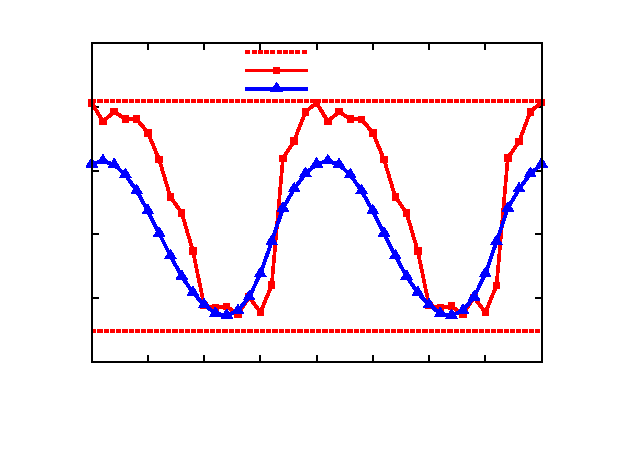
\includegraphics{sd_evo}}%
    \gplfronttext
  \end{picture}%
\endgroup
}
  \normalsize
  \caption{Normalized displacement velocity (red) and leading point location (blue) time history profiles at $100$ Hz.  The other two frequency cases show qualitatively the same evolution and are therefore not shown for clarity.}
  \label{fig:sd_evo}
\end{figure}


The normalized displacement velocities for the steady autoignition front and tribrachial flame are shown in Fig.~\ref{fig:sd_evo} as the top and bottom horizontal lines, respectively.  The $S_d/S_L$ for the steady tribrachial flame is around unity, while this value is around eight for the autoignition front.  These values are similar to those in HCCI combustion studies~\cite{yoo13} and therefore can be used to benchmark the unsteady cases.  The periodic time history profile of $S_d/S_L$ is bounded by but does not fully reach the two steady values, indicating that, while the chemical structure responds to the flow dynamics, such response is not fast enough to reach steady-state.  

When $S_d/S_L$ approaches the tribrachial flame limit, its value is almost constant, while the change near the autoignition limit is more sinusoidal.  Moreover, $S_d/S_L$ changes more abruptly when the combustion mode switches from tribrachial flame to autoignition.  Compared to the profile of the normalized leading point location ($x_d/D$), which is almost sinusoidal, the profile of the normalized displacement velocity is asymmetric, indicating that the transition from tribrachial flame to autoignition as the inlet velocity increases is not an exact reverse process of the transition from autoignition to tribrachial flame.  Indeed, as shown in Fig.~\ref{fig:HRR_100Hz}, although the inlet velocities at $0.25$ and $0.75$ cycle are the same, the structures demonstrate different morphologies during the cycle of decreasing and increasing velocity: there is hysteresis during the transition.

Such hysteresis is demonstrated more clearly in Fig.~\ref{fig:sd_hys}, where $S_d/S_L$ is plotted against the inlet velocity.  Qualitatively, all three oscillation frequency cases show similar trends: given the same inlet velocity, the reacting fronts have different displacement velocities during the cycle of decreasing and increasing velocity.  Additional evidence of hysteresis, shown in Fig.~\ref{fig:HRR_100Hz}, is the shift in the location of the leading point in the mixture fraction space: $Z = 0.14$ when the tribrachial flame dominates and $Z = 0.24$ when autoignition dominates.  The shift in the leading point mixture fraction as well as the displacement velocity indicates different dominant chemical reactions, and analysis of the dominant chemical reactions will reveal the mechanism of the hysteresis.

\begin{figure}[t]
  \centering
  \scriptsize
  \resizebox{0.5\textwidth}{!}{% GNUPLOT: LaTeX picture with Postscript
\begingroup
  \makeatletter
  \providecommand\color[2][]{%
    \GenericError{(gnuplot) \space\space\space\@spaces}{%
      Package color not loaded in conjunction with
      terminal option `colourtext'%
    }{See the gnuplot documentation for explanation.%
    }{Either use 'blacktext' in gnuplot or load the package
      color.sty in LaTeX.}%
    \renewcommand\color[2][]{}%
  }%
  \providecommand\includegraphics[2][]{%
    \GenericError{(gnuplot) \space\space\space\@spaces}{%
      Package graphicx or graphics not loaded%
    }{See the gnuplot documentation for explanation.%
    }{The gnuplot epslatex terminal needs graphicx.sty or graphics.sty.}%
    \renewcommand\includegraphics[2][]{}%
  }%
  \providecommand\rotatebox[2]{#2}%
  \@ifundefined{ifGPcolor}{%
    \newif\ifGPcolor
    \GPcolortrue
  }{}%
  \@ifundefined{ifGPblacktext}{%
    \newif\ifGPblacktext
    \GPblacktexttrue
  }{}%
  % define a \g@addto@macro without @ in the name:
  \let\gplgaddtomacro\g@addto@macro
  % define empty templates for all commands taking text:
  \gdef\gplbacktext{}%
  \gdef\gplfronttext{}%
  \makeatother
  \ifGPblacktext
    % no textcolor at all
    \def\colorrgb#1{}%
    \def\colorgray#1{}%
  \else
    % gray or color?
    \ifGPcolor
      \def\colorrgb#1{\color[rgb]{#1}}%
      \def\colorgray#1{\color[gray]{#1}}%
      \expandafter\def\csname LTw\endcsname{\color{white}}%
      \expandafter\def\csname LTb\endcsname{\color{black}}%
      \expandafter\def\csname LTa\endcsname{\color{black}}%
      \expandafter\def\csname LT0\endcsname{\color[rgb]{1,0,0}}%
      \expandafter\def\csname LT1\endcsname{\color[rgb]{0,1,0}}%
      \expandafter\def\csname LT2\endcsname{\color[rgb]{0,0,1}}%
      \expandafter\def\csname LT3\endcsname{\color[rgb]{1,0,1}}%
      \expandafter\def\csname LT4\endcsname{\color[rgb]{0,1,1}}%
      \expandafter\def\csname LT5\endcsname{\color[rgb]{1,1,0}}%
      \expandafter\def\csname LT6\endcsname{\color[rgb]{0,0,0}}%
      \expandafter\def\csname LT7\endcsname{\color[rgb]{1,0.3,0}}%
      \expandafter\def\csname LT8\endcsname{\color[rgb]{0.5,0.5,0.5}}%
    \else
      % gray
      \def\colorrgb#1{\color{black}}%
      \def\colorgray#1{\color[gray]{#1}}%
      \expandafter\def\csname LTw\endcsname{\color{white}}%
      \expandafter\def\csname LTb\endcsname{\color{black}}%
      \expandafter\def\csname LTa\endcsname{\color{black}}%
      \expandafter\def\csname LT0\endcsname{\color{black}}%
      \expandafter\def\csname LT1\endcsname{\color{black}}%
      \expandafter\def\csname LT2\endcsname{\color{black}}%
      \expandafter\def\csname LT3\endcsname{\color{black}}%
      \expandafter\def\csname LT4\endcsname{\color{black}}%
      \expandafter\def\csname LT5\endcsname{\color{black}}%
      \expandafter\def\csname LT6\endcsname{\color{black}}%
      \expandafter\def\csname LT7\endcsname{\color{black}}%
      \expandafter\def\csname LT8\endcsname{\color{black}}%
    \fi
  \fi
  \setlength{\unitlength}{0.0500bp}%
  \begin{picture}(5760.00,4032.00)%
    \gplgaddtomacro\gplbacktext{%
      \csname LTb\endcsname%
      \put(588,704){\makebox(0,0)[r]{\strut{} 0}}%
      \put(588,1317){\makebox(0,0)[r]{\strut{} 2}}%
      \put(588,1929){\makebox(0,0)[r]{\strut{} 4}}%
      \put(588,2542){\makebox(0,0)[r]{\strut{} 6}}%
      \put(588,3154){\makebox(0,0)[r]{\strut{} 8}}%
      \put(588,3767){\makebox(0,0)[r]{\strut{} 10}}%
      \put(720,484){\makebox(0,0){\strut{} 0}}%
      \put(1584,484){\makebox(0,0){\strut{} 2}}%
      \put(2448,484){\makebox(0,0){\strut{} 4}}%
      \put(3311,484){\makebox(0,0){\strut{} 6}}%
      \put(4175,484){\makebox(0,0){\strut{} 8}}%
      \put(5039,484){\makebox(0,0){\strut{} 10}}%
      \put(-50,2235){\rotatebox{-270}{\makebox(0,0){\strut{}\vspace{-28pt}$S_d/S_L$}}}%
      \put(2879,154){\makebox(0,0){\strut{}$U_{\rm inlet}$}}%
      \put(936,2695){\makebox(0,0)[l]{\strut{}Decreasing-velocity}}%
      \put(3527,1163){\makebox(0,0)[l]{\strut{}Increasing-velocity}}%
    }%
    \gplgaddtomacro\gplfronttext{%
      \csname LTb\endcsname%
      \put(1377,3618){\makebox(0,0)[r]{\strut{}Steady}}%
      \csname LTb\endcsname%
      \put(1377,3442){\makebox(0,0)[r]{\strut{}100 Hz}}%
      \csname LTb\endcsname%
      \put(1377,3266){\makebox(0,0)[r]{\strut{}50 Hz}}%
      \csname LTb\endcsname%
      \put(1377,3090){\makebox(0,0)[r]{\strut{}25 Hz}}%
    }%
    \gplbacktext
    \put(0,0){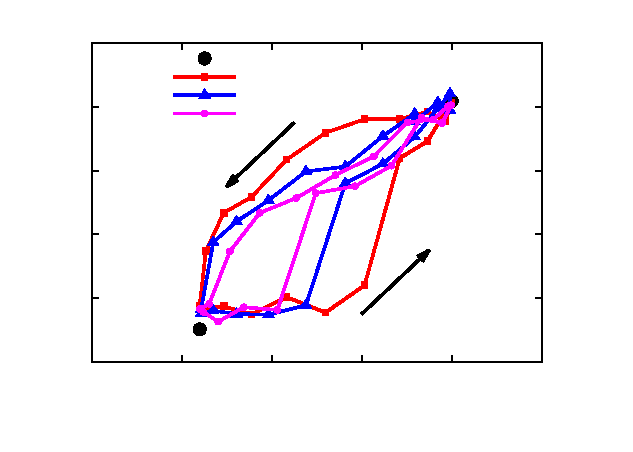
\includegraphics{sd_hys}}%
    \gplfronttext
  \end{picture}%
\endgroup
}
  \normalsize
  \vspace{-0.2in}
  \caption{Normalized displacement velocities at various inlet velocities for two steady cases and three oscillating unsteady cases.}
  \label{fig:sd_hys}
\end{figure}

From the steady case analysis~\cite{deng15b}, the dominant chemical pathways are found to be different at the leading point of the tribrachial flame and autoignition front.  Specifically, the hydrogen peroxide branching reaction (H$_2$O$_2$ + M $\Longleftrightarrow$ OH + OH + M) is the dominant chain branching reaction at the leading point of the autoignition front, while the H radical branching reaction (H + O$_2$ $\Longleftrightarrow$ O + OH) is the most important chain branching reaction at the tribrachial flame leading point.  Due to the longer residence time, hydrogen peroxide accumulation is much higher upstream of the autoignition front compared to the tribrachial flame front.  

\begin{figure}[t]
  \centering
  \scriptsize
  \resizebox{0.49\textwidth}{!}{% GNUPLOT: LaTeX picture with Postscript
\begingroup
  \makeatletter
  \providecommand\color[2][]{%
    \GenericError{(gnuplot) \space\space\space\@spaces}{%
      Package color not loaded in conjunction with
      terminal option `colourtext'%
    }{See the gnuplot documentation for explanation.%
    }{Either use 'blacktext' in gnuplot or load the package
      color.sty in LaTeX.}%
    \renewcommand\color[2][]{}%
  }%
  \providecommand\includegraphics[2][]{%
    \GenericError{(gnuplot) \space\space\space\@spaces}{%
      Package graphicx or graphics not loaded%
    }{See the gnuplot documentation for explanation.%
    }{The gnuplot epslatex terminal needs graphicx.sty or graphics.sty.}%
    \renewcommand\includegraphics[2][]{}%
  }%
  \providecommand\rotatebox[2]{#2}%
  \@ifundefined{ifGPcolor}{%
    \newif\ifGPcolor
    \GPcolortrue
  }{}%
  \@ifundefined{ifGPblacktext}{%
    \newif\ifGPblacktext
    \GPblacktexttrue
  }{}%
  % define a \g@addto@macro without @ in the name:
  \let\gplgaddtomacro\g@addto@macro
  % define empty templates for all commands taking text:
  \gdef\gplbacktext{}%
  \gdef\gplfronttext{}%
  \makeatother
  \ifGPblacktext
    % no textcolor at all
    \def\colorrgb#1{}%
    \def\colorgray#1{}%
  \else
    % gray or color?
    \ifGPcolor
      \def\colorrgb#1{\color[rgb]{#1}}%
      \def\colorgray#1{\color[gray]{#1}}%
      \expandafter\def\csname LTw\endcsname{\color{white}}%
      \expandafter\def\csname LTb\endcsname{\color{black}}%
      \expandafter\def\csname LTa\endcsname{\color{black}}%
      \expandafter\def\csname LT0\endcsname{\color[rgb]{1,0,0}}%
      \expandafter\def\csname LT1\endcsname{\color[rgb]{0,1,0}}%
      \expandafter\def\csname LT2\endcsname{\color[rgb]{0,0,1}}%
      \expandafter\def\csname LT3\endcsname{\color[rgb]{1,0,1}}%
      \expandafter\def\csname LT4\endcsname{\color[rgb]{0,1,1}}%
      \expandafter\def\csname LT5\endcsname{\color[rgb]{1,1,0}}%
      \expandafter\def\csname LT6\endcsname{\color[rgb]{0,0,0}}%
      \expandafter\def\csname LT7\endcsname{\color[rgb]{1,0.3,0}}%
      \expandafter\def\csname LT8\endcsname{\color[rgb]{0.5,0.5,0.5}}%
    \else
      % gray
      \def\colorrgb#1{\color{black}}%
      \def\colorgray#1{\color[gray]{#1}}%
      \expandafter\def\csname LTw\endcsname{\color{white}}%
      \expandafter\def\csname LTb\endcsname{\color{black}}%
      \expandafter\def\csname LTa\endcsname{\color{black}}%
      \expandafter\def\csname LT0\endcsname{\color{black}}%
      \expandafter\def\csname LT1\endcsname{\color{black}}%
      \expandafter\def\csname LT2\endcsname{\color{black}}%
      \expandafter\def\csname LT3\endcsname{\color{black}}%
      \expandafter\def\csname LT4\endcsname{\color{black}}%
      \expandafter\def\csname LT5\endcsname{\color{black}}%
      \expandafter\def\csname LT6\endcsname{\color{black}}%
      \expandafter\def\csname LT7\endcsname{\color{black}}%
      \expandafter\def\csname LT8\endcsname{\color{black}}%
    \fi
  \fi
  \setlength{\unitlength}{0.0500bp}%
  \begin{picture}(4320.00,3024.00)%
    \gplgaddtomacro\gplbacktext{%
      \csname LTb\endcsname%
      \put(948,704){\makebox(0,0)[r]{\strut{}0.0e+00}}%
      \put(948,1115){\makebox(0,0)[r]{\strut{}6.0e-03}}%
      \put(948,1526){\makebox(0,0)[r]{\strut{}1.2e-02}}%
      \put(948,1937){\makebox(0,0)[r]{\strut{}1.8e-02}}%
      \put(948,2348){\makebox(0,0)[r]{\strut{}2.4e-02}}%
      \put(948,2759){\makebox(0,0)[r]{\strut{}3.0e-02}}%
      \put(1080,484){\makebox(0,0){\strut{} 0}}%
      \put(1649,484){\makebox(0,0){\strut{} 2}}%
      \put(2217,484){\makebox(0,0){\strut{} 4}}%
      \put(2786,484){\makebox(0,0){\strut{} 6}}%
      \put(3354,484){\makebox(0,0){\strut{} 8}}%
      \put(3923,484){\makebox(0,0){\strut{} 10}}%
      \put(-218,1731){\rotatebox{-270}{\makebox(0,0){\strut{}\vspace{-28pt}$Y_{\rm H_2O_2}$}}}%
      \put(2501,154){\makebox(0,0){\strut{}$x/D$}}%
    }%
    \gplgaddtomacro\gplfronttext{%
      \csname LTb\endcsname%
      \put(2763,2603){\makebox(0,0)[r]{\strut{}Steady 2.4 m/s}}%
      \csname LTb\endcsname%
      \put(2763,2427){\makebox(0,0)[r]{\strut{}Steady 8.0 m/s}}%
      \csname LTb\endcsname%
      \put(2763,2251){\makebox(0,0)[r]{\strut{}0.25 cycle}}%
      \csname LTb\endcsname%
      \put(2763,2075){\makebox(0,0)[r]{\strut{}0.45 cycle}}%
      \csname LTb\endcsname%
      \put(2763,1899){\makebox(0,0)[r]{\strut{}0.5 cycle}}%
    }%
    \gplbacktext
    \put(0,0){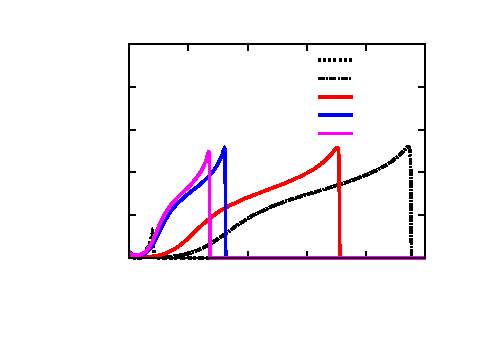
\includegraphics{H2O2_up}}%
    \gplfronttext
  \end{picture}%
\endgroup
}
  \resizebox{0.49\textwidth}{!}{% GNUPLOT: LaTeX picture with Postscript
\begingroup
  \makeatletter
  \providecommand\color[2][]{%
    \GenericError{(gnuplot) \space\space\space\@spaces}{%
      Package color not loaded in conjunction with
      terminal option `colourtext'%
    }{See the gnuplot documentation for explanation.%
    }{Either use 'blacktext' in gnuplot or load the package
      color.sty in LaTeX.}%
    \renewcommand\color[2][]{}%
  }%
  \providecommand\includegraphics[2][]{%
    \GenericError{(gnuplot) \space\space\space\@spaces}{%
      Package graphicx or graphics not loaded%
    }{See the gnuplot documentation for explanation.%
    }{The gnuplot epslatex terminal needs graphicx.sty or graphics.sty.}%
    \renewcommand\includegraphics[2][]{}%
  }%
  \providecommand\rotatebox[2]{#2}%
  \@ifundefined{ifGPcolor}{%
    \newif\ifGPcolor
    \GPcolortrue
  }{}%
  \@ifundefined{ifGPblacktext}{%
    \newif\ifGPblacktext
    \GPblacktexttrue
  }{}%
  % define a \g@addto@macro without @ in the name:
  \let\gplgaddtomacro\g@addto@macro
  % define empty templates for all commands taking text:
  \gdef\gplbacktext{}%
  \gdef\gplfronttext{}%
  \makeatother
  \ifGPblacktext
    % no textcolor at all
    \def\colorrgb#1{}%
    \def\colorgray#1{}%
  \else
    % gray or color?
    \ifGPcolor
      \def\colorrgb#1{\color[rgb]{#1}}%
      \def\colorgray#1{\color[gray]{#1}}%
      \expandafter\def\csname LTw\endcsname{\color{white}}%
      \expandafter\def\csname LTb\endcsname{\color{black}}%
      \expandafter\def\csname LTa\endcsname{\color{black}}%
      \expandafter\def\csname LT0\endcsname{\color[rgb]{1,0,0}}%
      \expandafter\def\csname LT1\endcsname{\color[rgb]{0,1,0}}%
      \expandafter\def\csname LT2\endcsname{\color[rgb]{0,0,1}}%
      \expandafter\def\csname LT3\endcsname{\color[rgb]{1,0,1}}%
      \expandafter\def\csname LT4\endcsname{\color[rgb]{0,1,1}}%
      \expandafter\def\csname LT5\endcsname{\color[rgb]{1,1,0}}%
      \expandafter\def\csname LT6\endcsname{\color[rgb]{0,0,0}}%
      \expandafter\def\csname LT7\endcsname{\color[rgb]{1,0.3,0}}%
      \expandafter\def\csname LT8\endcsname{\color[rgb]{0.5,0.5,0.5}}%
    \else
      % gray
      \def\colorrgb#1{\color{black}}%
      \def\colorgray#1{\color[gray]{#1}}%
      \expandafter\def\csname LTw\endcsname{\color{white}}%
      \expandafter\def\csname LTb\endcsname{\color{black}}%
      \expandafter\def\csname LTa\endcsname{\color{black}}%
      \expandafter\def\csname LT0\endcsname{\color{black}}%
      \expandafter\def\csname LT1\endcsname{\color{black}}%
      \expandafter\def\csname LT2\endcsname{\color{black}}%
      \expandafter\def\csname LT3\endcsname{\color{black}}%
      \expandafter\def\csname LT4\endcsname{\color{black}}%
      \expandafter\def\csname LT5\endcsname{\color{black}}%
      \expandafter\def\csname LT6\endcsname{\color{black}}%
      \expandafter\def\csname LT7\endcsname{\color{black}}%
      \expandafter\def\csname LT8\endcsname{\color{black}}%
    \fi
  \fi
  \setlength{\unitlength}{0.0500bp}%
  \begin{picture}(4320.00,3024.00)%
    \gplgaddtomacro\gplbacktext{%
      \csname LTb\endcsname%
      \put(948,704){\makebox(0,0)[r]{\strut{}0.0e+00}}%
      \put(948,1115){\makebox(0,0)[r]{\strut{}6.0e-03}}%
      \put(948,1526){\makebox(0,0)[r]{\strut{}1.2e-02}}%
      \put(948,1937){\makebox(0,0)[r]{\strut{}1.8e-02}}%
      \put(948,2348){\makebox(0,0)[r]{\strut{}2.4e-02}}%
      \put(948,2759){\makebox(0,0)[r]{\strut{}3.0e-02}}%
      \put(1080,484){\makebox(0,0){\strut{} 0}}%
      \put(1649,484){\makebox(0,0){\strut{} 2}}%
      \put(2217,484){\makebox(0,0){\strut{} 4}}%
      \put(2786,484){\makebox(0,0){\strut{} 6}}%
      \put(3354,484){\makebox(0,0){\strut{} 8}}%
      \put(3923,484){\makebox(0,0){\strut{} 10}}%
      \put(-218,1731){\rotatebox{-270}{\makebox(0,0){\strut{}\vspace{-28pt}$Y_{\rm H_2O_2}$}}}%
      \put(2501,154){\makebox(0,0){\strut{}$x/D$}}%
    }%
    \gplgaddtomacro\gplfronttext{%
      \csname LTb\endcsname%
      \put(2479,2603){\makebox(0,0)[r]{\strut{}Steady 2.4 m/s}}%
      \csname LTb\endcsname%
      \put(2479,2427){\makebox(0,0)[r]{\strut{}Steady 8.0 m/s}}%
      \csname LTb\endcsname%
      \put(2479,2251){\makebox(0,0)[r]{\strut{}0.5 cycle}}%
      \csname LTb\endcsname%
      \put(2479,2075){\makebox(0,0)[r]{\strut{}0.55 cycle}}%
      \csname LTb\endcsname%
      \put(2479,1899){\makebox(0,0)[r]{\strut{}0.65 cycle}}%
      \csname LTb\endcsname%
      \put(2479,1723){\makebox(0,0)[r]{\strut{}0.75 cycle}}%
      \csname LTb\endcsname%
      \put(2479,1547){\makebox(0,0)[r]{\strut{}0.85 cycle}}%
    }%
    \gplbacktext
    \put(0,0){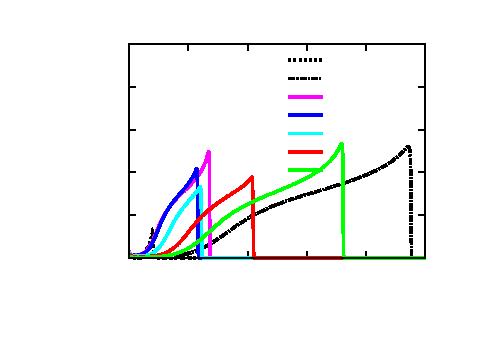
\includegraphics{H2O2_down}}%
    \gplfronttext
  \end{picture}%
\endgroup
}
  \vspace{-0.2in}
  \normalsize
  \caption{The comparison of hydrogen peroxide mass fraction profiles along the $Z = 0.24$ iso-contour at steady state and at $100$ Hz during the decreasing-velocity cycle (left) and increasing-velocity cycle (right).}
  \label{fig:H2O2_updown}
\end{figure}

As hydrogen peroxide plays different roles in the tribrachial flame and autoignition front, its spatial profiles along the $Z = 0.24$ iso-contour are compared in Fig.~\ref{fig:H2O2_updown}, with the left and right subfigures corresponding to the decreasing-velocity and increasing-velocity half cycles, respectively.  The left figure shows that hydrogen peroxide keeps on accumulating until either autoignition occurs or it is consumed at the flame front, resulting in a sharp drop in its mass fraction.  However, the peak value of the hydrogen peroxide mass fraction differs by five times between a steady autoignition front and tribrachial flame, which implies its different significance in these two combustion modes and sets the benchmark for the unsteady evolution.  As the inlet velocity decreases from $8.0$ m/s, the peak $Y_{\rm H{_2}O{_2}}$ almost remains constant, indicating that the chemical structure is very close to the steady autoignition case.  As a consequence, the dominant chemical pathway remains as H$_2$O$_2$ + M $\Longleftrightarrow$ OH + OH + M, and autoignition is the dominant combustion process, resulting in larger $S_d/S_L$.  However, as the flow velocity decreases, a larger gradient is achieved, resulting in steeper profiles and smaller $S_d/S_L$, according to Eq.~(\ref{eq:sd}).       

Even when the inlet velocity reaches the minimum $2.4$ m/s, which is the same as the steady case, the reacting front continues to move upstream.  Inlet velocity changes slowest around the half cycle, allowing the chemical structure to respond to the hydrodynamic changes.  As shown on the right of Fig.~\ref{fig:H2O2_updown}, the peak $Y_{\rm H{_2}O{_2}}$ decreases from $0.5$ to $0.65$ of the cycle.  At this stage, autoignition is not fully activated, since the peak $Y_{\rm H{_2}O{_2}}$ is lower than the steady autoignition case.  However, the peak $Y_{\rm H{_2}O{_2}}$ is still larger than the steady tribrachial flame.  Therefore, the $S_d/S_L$ of the tribrachial structure is close to but slightly larger than a steady flame, for it is propagating into a partially reacted mixture.  

This tribrachial structure is convected downstream, as inlet velocity further increases from $0.65$ to $0.75$ of the cycle.  The unburnt mixture upstream of the flame accumulates radicals and heat as it moves downstream.  It finally autoignites, denoted by a sudden jump of $S_d/S_L$.  

\subsection{Effects of oscillation frequency}

Compared to the $100$ Hz case, the other two cases of lower oscillation frequency are similar qualitatively but with some quantitative differences.  As shown in Fig.~\ref{fig:sd_hys}, the hysteresis of decreasing and increasing velocity is diminished as the oscillation frequency decreases, denoted by the shrinking of the enclosed area.  Hysteresis remains at slower inlet velocities since the decreasing-velocity branch is still autoignition dominated, but it takes finite induction time for the increasing-velocity unburnt mixture to achieve autoignition.  At higher inlet velocities, both branches are autoignition dominant and therefore collapse to a single path at sufficiently low frequency, approaching the quasi-steady limit.

The $100$ Hz case demonstrates hysteresis for a relatively larger portion of its oscillation cycle.  However, the time intervals between sampling points in Fig.~\ref{fig:sd_hys} are not the same for the three frequencies, being $0.5$, $1.0$, and $2.0$ ms for 100, 50, and 25 Hz, respectively. Therefore, in terms of absolute time, the $25$ Hz case takes a longer time to achieve the transition from small $S_d/S_L$ to larger values during the increasing-velocity portion of the cycle, indicating a longer induction time.  

This counter-intuitive finding is explained with Fig.~\ref{fig:species_frq}.  Here, the hydrogen peroxide profiles are compared for three frequency cases for both decreasing and increasing-velocity branches, at the same inlet velocity of $3.2$ m/s, and benchmarked with the corresponding steady computation.  According to previous studies~\cite{deng15,deng15b}, this steady case is autoignition dominated at $Z = 0.24$.  Three unsteady profiles on the decreasomg-velocity branch show similar peak values, and, the lower the frequency, the closer the profile matches the steady case, which is expected.  However, the unsteady profiles on the increasing-velocity branch show lower peak values than the steady structure.  Moreover, the $100$ Hz case profile is closer to the steady counterpart.  Noting from Fig.~\ref{fig:sd_hys} that the minimum $S_d/S_L$ in all three cases are larger than the steady $2.4$ m/s case and at lower frequency the unburnt mixture has longer time to relax to steady state, the $25$ Hz case should match the $2.4$ m/s steady case closer, that is, a tribrachial flame with low H$_2$O$_2$ accumulation.  Therefore, it takes longer time to accumulate sufficient hydrogen peroxide to activate autoignition.  Conversely, the $100$ Hz case allows less time to relax to a steady flame structure and therefore has larger $Y_{\rm H_2O_2}$ to start with during the increasing-velocity cycle, resulting in a shorter induction time for autoignition.

\begin{figure}[t]
  \centering
  \scriptsize
  \resizebox{0.49\textwidth}{!}{% GNUPLOT: LaTeX picture with Postscript
\begingroup
  \makeatletter
  \providecommand\color[2][]{%
    \GenericError{(gnuplot) \space\space\space\@spaces}{%
      Package color not loaded in conjunction with
      terminal option `colourtext'%
    }{See the gnuplot documentation for explanation.%
    }{Either use 'blacktext' in gnuplot or load the package
      color.sty in LaTeX.}%
    \renewcommand\color[2][]{}%
  }%
  \providecommand\includegraphics[2][]{%
    \GenericError{(gnuplot) \space\space\space\@spaces}{%
      Package graphicx or graphics not loaded%
    }{See the gnuplot documentation for explanation.%
    }{The gnuplot epslatex terminal needs graphicx.sty or graphics.sty.}%
    \renewcommand\includegraphics[2][]{}%
  }%
  \providecommand\rotatebox[2]{#2}%
  \@ifundefined{ifGPcolor}{%
    \newif\ifGPcolor
    \GPcolortrue
  }{}%
  \@ifundefined{ifGPblacktext}{%
    \newif\ifGPblacktext
    \GPblacktexttrue
  }{}%
  % define a \g@addto@macro without @ in the name:
  \let\gplgaddtomacro\g@addto@macro
  % define empty templates for all commands taking text:
  \gdef\gplbacktext{}%
  \gdef\gplfronttext{}%
  \makeatother
  \ifGPblacktext
    % no textcolor at all
    \def\colorrgb#1{}%
    \def\colorgray#1{}%
  \else
    % gray or color?
    \ifGPcolor
      \def\colorrgb#1{\color[rgb]{#1}}%
      \def\colorgray#1{\color[gray]{#1}}%
      \expandafter\def\csname LTw\endcsname{\color{white}}%
      \expandafter\def\csname LTb\endcsname{\color{black}}%
      \expandafter\def\csname LTa\endcsname{\color{black}}%
      \expandafter\def\csname LT0\endcsname{\color[rgb]{1,0,0}}%
      \expandafter\def\csname LT1\endcsname{\color[rgb]{0,1,0}}%
      \expandafter\def\csname LT2\endcsname{\color[rgb]{0,0,1}}%
      \expandafter\def\csname LT3\endcsname{\color[rgb]{1,0,1}}%
      \expandafter\def\csname LT4\endcsname{\color[rgb]{0,1,1}}%
      \expandafter\def\csname LT5\endcsname{\color[rgb]{1,1,0}}%
      \expandafter\def\csname LT6\endcsname{\color[rgb]{0,0,0}}%
      \expandafter\def\csname LT7\endcsname{\color[rgb]{1,0.3,0}}%
      \expandafter\def\csname LT8\endcsname{\color[rgb]{0.5,0.5,0.5}}%
    \else
      % gray
      \def\colorrgb#1{\color{black}}%
      \def\colorgray#1{\color[gray]{#1}}%
      \expandafter\def\csname LTw\endcsname{\color{white}}%
      \expandafter\def\csname LTb\endcsname{\color{black}}%
      \expandafter\def\csname LTa\endcsname{\color{black}}%
      \expandafter\def\csname LT0\endcsname{\color{black}}%
      \expandafter\def\csname LT1\endcsname{\color{black}}%
      \expandafter\def\csname LT2\endcsname{\color{black}}%
      \expandafter\def\csname LT3\endcsname{\color{black}}%
      \expandafter\def\csname LT4\endcsname{\color{black}}%
      \expandafter\def\csname LT5\endcsname{\color{black}}%
      \expandafter\def\csname LT6\endcsname{\color{black}}%
      \expandafter\def\csname LT7\endcsname{\color{black}}%
      \expandafter\def\csname LT8\endcsname{\color{black}}%
    \fi
  \fi
  \setlength{\unitlength}{0.0500bp}%
  \begin{picture}(4320.00,3024.00)%
    \gplgaddtomacro\gplbacktext{%
      \csname LTb\endcsname%
      \put(948,704){\makebox(0,0)[r]{\strut{}0.0e+00}}%
      \put(948,1115){\makebox(0,0)[r]{\strut{}6.0e-03}}%
      \put(948,1526){\makebox(0,0)[r]{\strut{}1.2e-02}}%
      \put(948,1937){\makebox(0,0)[r]{\strut{}1.8e-02}}%
      \put(948,2348){\makebox(0,0)[r]{\strut{}2.4e-02}}%
      \put(948,2759){\makebox(0,0)[r]{\strut{}3.0e-02}}%
      \put(1080,484){\makebox(0,0){\strut{} 0}}%
      \put(1649,484){\makebox(0,0){\strut{} 1}}%
      \put(2217,484){\makebox(0,0){\strut{} 2}}%
      \put(2786,484){\makebox(0,0){\strut{} 3}}%
      \put(3354,484){\makebox(0,0){\strut{} 4}}%
      \put(3923,484){\makebox(0,0){\strut{} 5}}%
      \put(-218,1731){\rotatebox{-270}{\makebox(0,0){\strut{}\vspace{-28pt}$Y_{\rm H_2O_2}$}}}%
      \put(2501,154){\makebox(0,0){\strut{}$x/D$}}%
    }%
    \gplgaddtomacro\gplfronttext{%
      \csname LTb\endcsname%
      \put(1960,2603){\makebox(0,0)[r]{\strut{}Steady 3.2 m/s}}%
      \csname LTb\endcsname%
      \put(1960,2427){\makebox(0,0)[r]{\strut{}100 Hz DV}}%
      \csname LTb\endcsname%
      \put(1960,2251){\makebox(0,0)[r]{\strut{}50 Hz DV}}%
      \csname LTb\endcsname%
      \put(1960,2075){\makebox(0,0)[r]{\strut{}25 Hz DV}}%
      \csname LTb\endcsname%
      \put(1960,1899){\makebox(0,0)[r]{\strut{}100 Hz IV}}%
      \csname LTb\endcsname%
      \put(1960,1723){\makebox(0,0)[r]{\strut{}50 Hz IV}}%
      \csname LTb\endcsname%
      \put(1960,1547){\makebox(0,0)[r]{\strut{}25 Hz IV}}%
    }%
    \gplbacktext
    \put(0,0){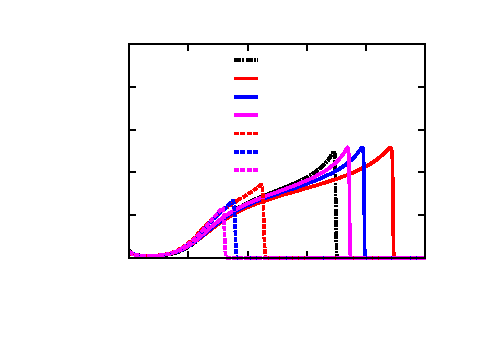
\includegraphics{H2O2_32}}%
    \gplfronttext
  \end{picture}%
\endgroup
}
  \resizebox{0.49\textwidth}{!}{% GNUPLOT: LaTeX picture with Postscript
\begingroup
  \makeatletter
  \providecommand\color[2][]{%
    \GenericError{(gnuplot) \space\space\space\@spaces}{%
      Package color not loaded in conjunction with
      terminal option `colourtext'%
    }{See the gnuplot documentation for explanation.%
    }{Either use 'blacktext' in gnuplot or load the package
      color.sty in LaTeX.}%
    \renewcommand\color[2][]{}%
  }%
  \providecommand\includegraphics[2][]{%
    \GenericError{(gnuplot) \space\space\space\@spaces}{%
      Package graphicx or graphics not loaded%
    }{See the gnuplot documentation for explanation.%
    }{The gnuplot epslatex terminal needs graphicx.sty or graphics.sty.}%
    \renewcommand\includegraphics[2][]{}%
  }%
  \providecommand\rotatebox[2]{#2}%
  \@ifundefined{ifGPcolor}{%
    \newif\ifGPcolor
    \GPcolortrue
  }{}%
  \@ifundefined{ifGPblacktext}{%
    \newif\ifGPblacktext
    \GPblacktexttrue
  }{}%
  % define a \g@addto@macro without @ in the name:
  \let\gplgaddtomacro\g@addto@macro
  % define empty templates for all commands taking text:
  \gdef\gplbacktext{}%
  \gdef\gplfronttext{}%
  \makeatother
  \ifGPblacktext
    % no textcolor at all
    \def\colorrgb#1{}%
    \def\colorgray#1{}%
  \else
    % gray or color?
    \ifGPcolor
      \def\colorrgb#1{\color[rgb]{#1}}%
      \def\colorgray#1{\color[gray]{#1}}%
      \expandafter\def\csname LTw\endcsname{\color{white}}%
      \expandafter\def\csname LTb\endcsname{\color{black}}%
      \expandafter\def\csname LTa\endcsname{\color{black}}%
      \expandafter\def\csname LT0\endcsname{\color[rgb]{1,0,0}}%
      \expandafter\def\csname LT1\endcsname{\color[rgb]{0,1,0}}%
      \expandafter\def\csname LT2\endcsname{\color[rgb]{0,0,1}}%
      \expandafter\def\csname LT3\endcsname{\color[rgb]{1,0,1}}%
      \expandafter\def\csname LT4\endcsname{\color[rgb]{0,1,1}}%
      \expandafter\def\csname LT5\endcsname{\color[rgb]{1,1,0}}%
      \expandafter\def\csname LT6\endcsname{\color[rgb]{0,0,0}}%
      \expandafter\def\csname LT7\endcsname{\color[rgb]{1,0.3,0}}%
      \expandafter\def\csname LT8\endcsname{\color[rgb]{0.5,0.5,0.5}}%
    \else
      % gray
      \def\colorrgb#1{\color{black}}%
      \def\colorgray#1{\color[gray]{#1}}%
      \expandafter\def\csname LTw\endcsname{\color{white}}%
      \expandafter\def\csname LTb\endcsname{\color{black}}%
      \expandafter\def\csname LTa\endcsname{\color{black}}%
      \expandafter\def\csname LT0\endcsname{\color{black}}%
      \expandafter\def\csname LT1\endcsname{\color{black}}%
      \expandafter\def\csname LT2\endcsname{\color{black}}%
      \expandafter\def\csname LT3\endcsname{\color{black}}%
      \expandafter\def\csname LT4\endcsname{\color{black}}%
      \expandafter\def\csname LT5\endcsname{\color{black}}%
      \expandafter\def\csname LT6\endcsname{\color{black}}%
      \expandafter\def\csname LT7\endcsname{\color{black}}%
      \expandafter\def\csname LT8\endcsname{\color{black}}%
    \fi
  \fi
  \setlength{\unitlength}{0.0500bp}%
  \begin{picture}(5760.00,3024.00)%
    \gplgaddtomacro\gplbacktext{%
      \csname LTb\endcsname%
      \put(948,704){\makebox(0,0)[r]{\strut{}0.0e+00}}%
      \put(948,1115){\makebox(0,0)[r]{\strut{}7.0e-04}}%
      \put(948,1526){\makebox(0,0)[r]{\strut{}1.4e-03}}%
      \put(948,1937){\makebox(0,0)[r]{\strut{}2.1e-03}}%
      \put(948,2348){\makebox(0,0)[r]{\strut{}2.8e-03}}%
      \put(948,2759){\makebox(0,0)[r]{\strut{}3.5e-03}}%
      \put(1080,484){\makebox(0,0){\strut{} 0}}%
      \put(1937,484){\makebox(0,0){\strut{} 1}}%
      \put(2793,484){\makebox(0,0){\strut{} 2}}%
      \put(3650,484){\makebox(0,0){\strut{} 3}}%
      \put(4506,484){\makebox(0,0){\strut{} 4}}%
      \put(5363,484){\makebox(0,0){\strut{} 5}}%
      \put(-218,1731){\rotatebox{-270}{\makebox(0,0){\strut{}\vspace{-28pt}$Y_{\rm CH_3OCH_2O_2}$}}}%
      \put(3221,154){\makebox(0,0){\strut{}$x/D$}}%
    }%
    \gplgaddtomacro\gplfronttext{%
      \csname LTb\endcsname%
      \put(4707,2473){\makebox(0,0)[r]{\strut{}Steady 3.2 m/s}}%
      \csname LTb\endcsname%
      \put(4707,2253){\makebox(0,0)[r]{\strut{}100 Hz DV}}%
      \csname LTb\endcsname%
      \put(4707,2033){\makebox(0,0)[r]{\strut{}50 Hz DV}}%
      \csname LTb\endcsname%
      \put(4707,1813){\makebox(0,0)[r]{\strut{}25 Hz DV}}%
      \csname LTb\endcsname%
      \put(4707,1593){\makebox(0,0)[r]{\strut{}100 Hz IV}}%
      \csname LTb\endcsname%
      \put(4707,1373){\makebox(0,0)[r]{\strut{}50 Hz IV}}%
      \csname LTb\endcsname%
      \put(4707,1153){\makebox(0,0)[r]{\strut{}25 Hz IV}}%
    }%
    \gplbacktext
    \put(0,0){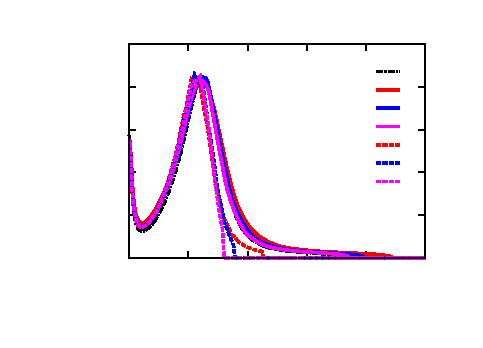
\includegraphics{RO2_32}}%
    \gplfronttext
  \end{picture}%
\endgroup
}
  \normalsize
  \vspace{-0.2in}
  \caption{Hydrogen peroxide and methyoxymethylperoxy radical mass fraction profiles along the $Z = 0.24$ iso-contour at $3.2$ m/s.  DV: decreasing-velocity, and IV: increasing-velocity.}
  \label{fig:species_frq}
\end{figure}

As demonstrated in previous studies~\cite{deng15,deng15b}, NTC chemistry is important in the upstream of both tribrachial flame and autoignition front.  The methoxymethylperoxy radical (CH$_3$OCH$_2$O$_2$) is chosen to represent the NTC chemistry~\cite{krisman14}, and its mass fraction profiles are shown in Fig.~\ref{fig:species_frq} to elucidate the effects of the oscillation frequency.  It is seen that irrespective of the oscillation frequency and traveling direction, at the same inlet velocity, $Y_{\rm CH_3OCH_2O_2}$ matches with its steady state profile.  Compared to the distinct behavior of $Y_{\rm H_2O_2}$, it is seen that the NTC chemistry time scale is relatively short compared to the accumulation of hydrogen peroxide.  The induction time for the first-stage ignition facilitated by NTC chemistry is relatively short ($\sim 0.3$ ms~\cite{deng15b}) compared to the major autoignition process induced by the hydrogen peroxide branching reaction ($\sim 1$ ms~\cite{deng15b}) and the characteristic hydrodynamic oscillation time ($10$-$40$ ms in the current work).  Therefore, NTC chemistry can be decoupled from flow dynamics.  Conversely, the coupling between fluid dynamics and second-stage autoignition/flame is important.       


%====================================================================

\section{Conclusions}

Axisymmetric laminar nonpremixed DME coflow flames at elevated temperatures and pressures with sinusoidally oscillating inlet velocities were computationally investigated.  The inlet velocity oscillates between $2.4$ and $8.0$ m/s at $25$, $50$, and $100$ Hz.  Flame dynamics in such oscillating flows and frequency effects on the hydrodynamics-chemistry coupling were analyzed.

The heat release rate profiles were examined to describe the thermal structure.  The morphology of the thermal structure transitions between tribrachial and multibrachial.  The multibrachial structure is favored when the inlet velocity is higher, although there is hysteresis during the transition.  Such structures agree well with the steady cases in Deng~\emph{et al.}~\cite{deng15b}, which correspond to different combustion modes: tribrachial flame and autoignition.  Normalized displacement velocity was defined to differentiate these two modes in the current study and compare with the steady cases.  

According to the steady results, the normalized displacement velocity for a tribrachial flame is around unity and is larger for autoignition.  The same criterion was applied to the unsteady cases to elucidate the evolution of combustion mode.  As the inlet velocity decreases, autoignition is the dominant combustion process until flame chemistry takes over around the most upstream location and slowest inlet velocity.  The tribrachial flame is convected downstream as the flow velocity increases.  The radical and heat accumulation upstream of the tribrachial flame finally results in autoignition, showing a sudden increase in the normalized displacement velocity.  

Examining the evolution of methyoxymethylperoxy radical and hydrogen peroxide profiles during the oscillation process, it is found that, at the three frequencies investigated, the tribrachial structure does not have sufficient time to reach steady state.  Consequently, the decreasing-velocity and increasing-velocity cycles have different normalized displacement velocities and hence demonstrate hysteresis.  NTC chemistry represented by methyoxymethylperoxy radical accumulation and depletion has shorter time scales and therefore is able to respond to the hydrodynamic changes.  However, autoignition and flame establishment have comparable time scales to the oscillation periods, and the lower frequency case is closer to reaching the steady state condition.

\section*{Acknowledgments}
This research was supported in part by the Air Force Office of Scientific Research (AFOSR) under the technical management of Dr. Mitat Birkan.

%====================================================================

\section*{References}
\bibliographystyle{elsarticle-num-PCI}
\bibliography{unsteady}

\renewcommand{\thefigure}{\arabic{figure}}
\renewcommand{\thetable}{\arabic{table}}

\clearpage
\listoffigures

\end{document}





  
